\documentclass[11pt,a4paper]{article}

%%%%%%%%%%%%%%%%%%

\thispagestyle{empty}

\usepackage{latexsym}
\usepackage{amssymb}
\usepackage{amsmath}
\usepackage{amsfonts}
\usepackage{color}
\usepackage{graphicx}
\usepackage{epsfig}
\usepackage{epstopdf}
\usepackage{amsthm}

\usepackage{subcaption}
\usepackage{tikz}
\usepackage{tkz-fct}
%%%%%%%%%%%%%%%%%%

\usepackage[spanish]{babel}
\usepackage[utf8]{inputenc}

\newcommand{\blue}{\textcolor{blue}}
\newcommand{\red}{\textcolor{red}}
\newcommand{\w}{\textcolor{white}}

%%%%%%%%%%%%%%%%%%

\addtolength{\topmargin}{-3cm} 
\addtolength{\oddsidemargin}{-2.5cm}
\addtolength{\textheight}{+5cm} 
\addtolength{\textwidth}{+5cm}


\parindent=0cm    
\parskip=0mm

%%%%%%%%%%%%%%%%%%



\begin{document}
\hrule\hrule
\vspace{2mm}

\noindent {\bf Fundamentos de Análisis Matemático, MMA 2024-25.
\hfill{ENTREGA 2}}

\vspace{3mm}

 \noindent {\bf NOMBRE}: Gonzalo Ortega Carpintero \hfill ({\it Para entregar el jueves, 1 de noviembre})

\vspace{2mm}

\hrule\hrule 

\vspace{2mm}

\

%{\sc The following exercise gives simple proofs of Urysohn's Lemma in $\mathbb R^N$}:

\vskip 3mm

\noindent  {\bf 1.} Sea $M$ el operador maximal centrado de Hardy-Littlewood, es decir
$$
Mf(x)=\sup_{r>0} \frac 1{|B_r|}\int_{B_r(x)}|f(y)|\, dy.
$$
Mostrar que si $f\in L^1(\mathbb R^n)$ entonces $Mf\notin L^1(\mathbb R^n)$ a menos que $f=0$ a.e.
\vskip 2mm
%HINT:  Prove that $Mf(x)\ge c_0\frac 1{|x-z|^n}$ for some $z\in \mathbb R^n$ and some $c_0>0$ (both depending on $f$) and  {} \hskip 14mm for all $x\in \mathbb R^n$ with $|x-z|>1$.

\vskip 6mm

 \noindent {\bf 2.} Con un poco de imaginación, y suponiendo que la foto adjunta representa los primeros pasos de la construcción de una figura fractal semejante a la del triángulo de Sierpinski, determina (sin demostración) su dimensión de Hausdorff.
 \begin{figure}[h] 
   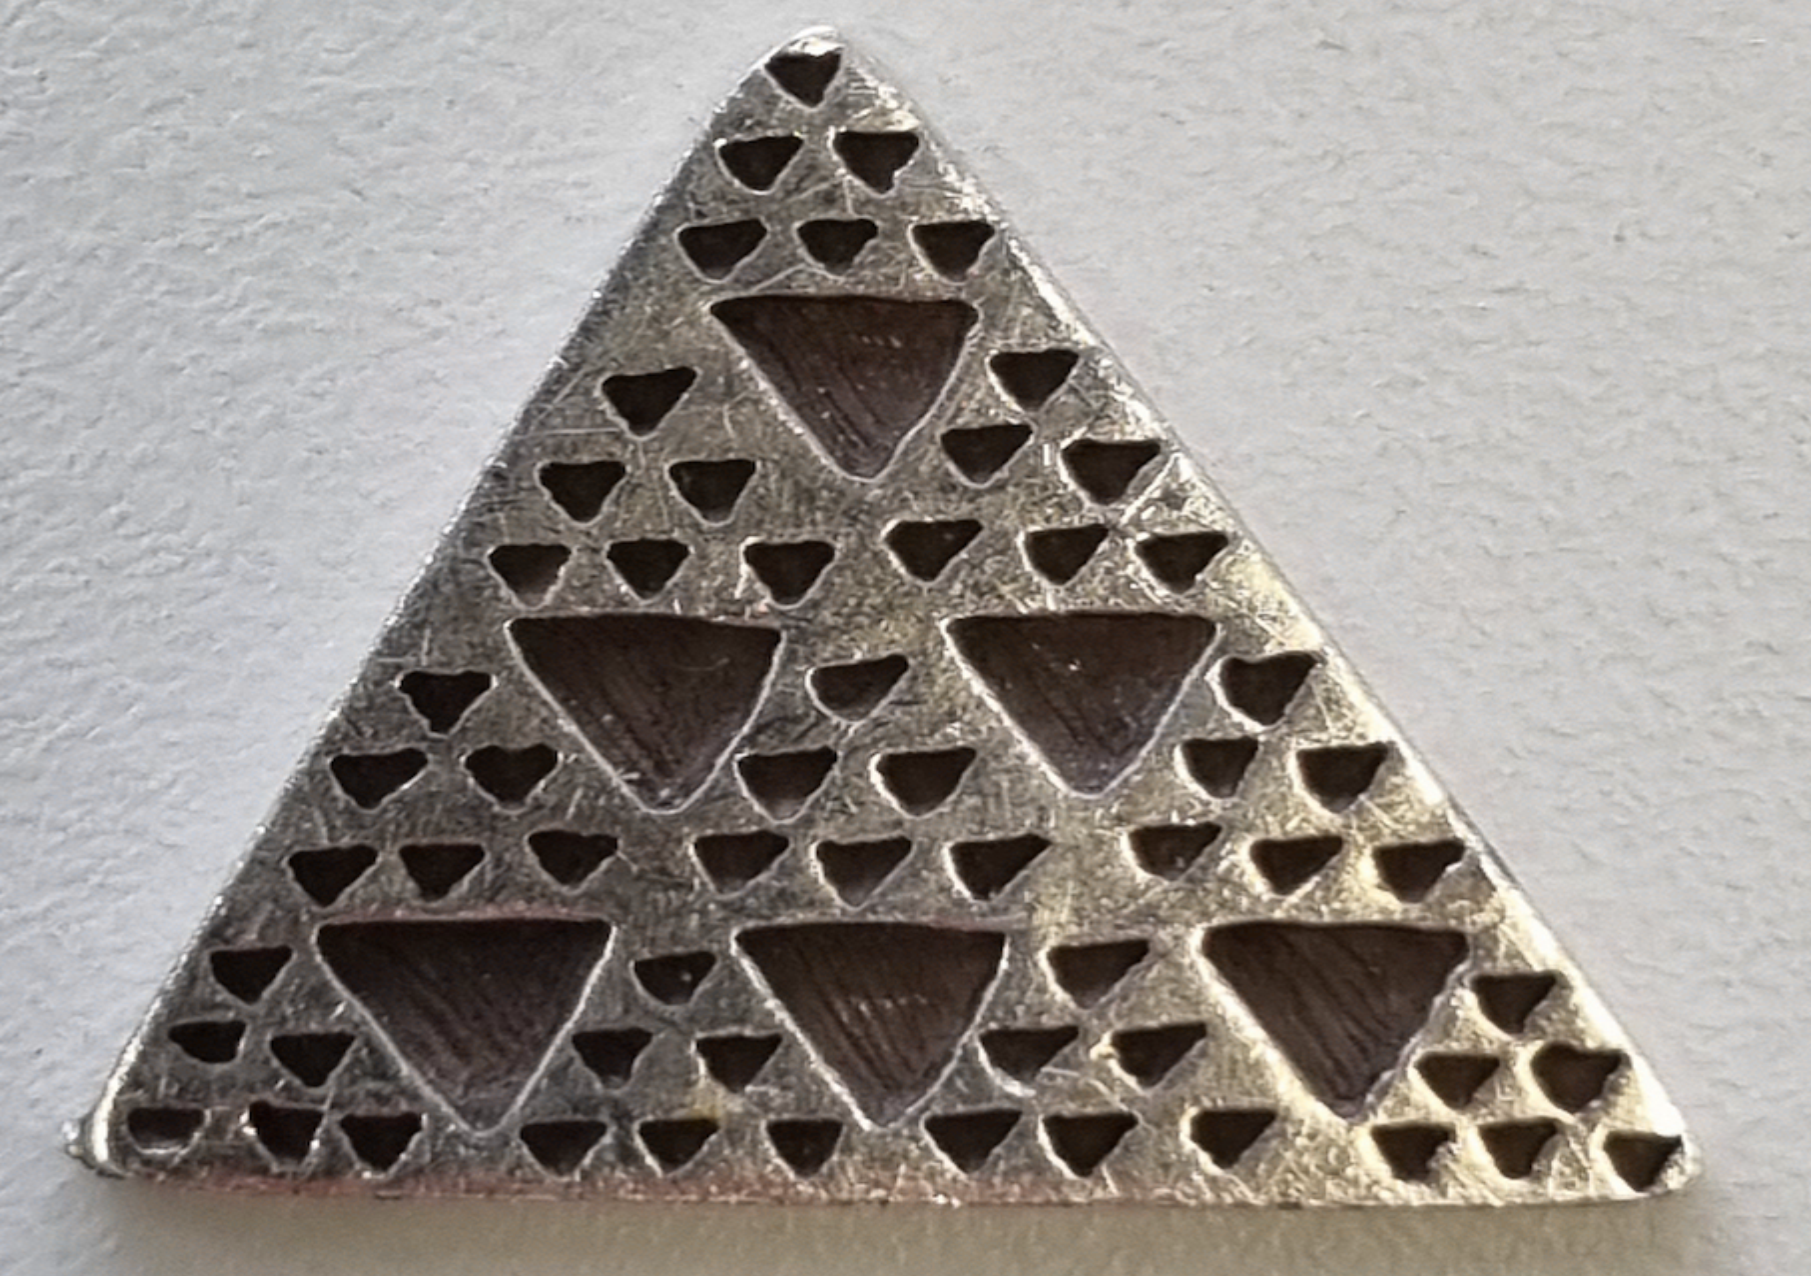
\includegraphics[width=80mm, height=60mm] {triangle.png}    
\end{figure}

 
 
 
 \vskip 6mm

 \noindent {\bf 3.}   Demuestra que si $R_j$ es una colección de rectángulos centrados en el origen del plano $\mathbb R^2$ con la propiedad de que $\displaystyle \lim_{j\to\infty} \mbox{diag}(R_j)= 0,$ entonces, si $1<p<\infty$ y $f\in L^p(\mathbb R^2)$ se tiene
 $$
 \lim_{j\to\infty}\frac 1{|R_j|}\int_{R_j} f(x-y)\, dy = f(x), \quad \mbox{a.e. }  x.
 $$
 {\it Indicación}: Pruébalo primero para funciones continuas con soporte compacto y luego demuestra (y usa a continuación) que el operador maximal, $M_s$, sobre ese tipo de rectángulos está acotado por la composición de dos operadores maximales unidimensionales de Hardy-Littlewood $M_1, \, M_2$ de la forma
 $$
 M_1f(x_1,x_2)=\sup_{h>0}\; \frac1{2h}\int_{-h}^{h}|f(x_1-t,x_2)|\, dt.
 $$
 (De forma similar se define $M_2$.)
   
\vskip 6mm
\hrule
\vskip 5mm

\newpage
\noindent {\bf SOL.:} 

\subsection*{1.}
\begin{proof}
  Si fuera $ f = 0 $ a.e., entonces $ Mf(x) = 0 $ a.e. y se tendría
  $$
    \| Mf(x) \|_{L^1} = \int_{\mathbb R^n} |Mf(x)| dx = 0 < \infty.
  $$
  Si $ f \neq 0 $ a.e., entonces para cualquier $ x \in \mathbb R^n $ podemos tomar un $ z \in \mathbb R^n $ que cumpla que $ |x-z| > 1$ y que en un entorno de $ z $, exista algún $ y \in \mathbb R^n $ de forma que $ f(y) \neq 0 $. Así, para una bola centrada en $ x $ de radio $ |x-z| $, la integral 
  $
    \int_{B_{|x-z|}} |f(y)|\, dy > 0.
  $
  Por otro lado tenemos que el volumen la bola n-dimensional se puede expresar como
  $ |B_r| = \frac{1}{c_n} r^n $, para un $c_n > 0 $. Así, tomando $ r = |x-z| $ en la definición del operador maximal, tenemos que
  $$
    Mf(x) \geq \frac{1}{|B_{|x-z|}|} \int_{B_{|x-z|}(x)} |f(y)|\, dy \geq c_n \frac{1}{|x-z|^n} \int_{B_{|x-z|}(x)} |f(y)|\, dy \geq c_n \frac{1}{|x-z|^n}.
  $$
  Integrando a ambos lados y haciendo el cambio de variable $ u = x - z $, de forma que $ du = dz $, tenemos
  $$
    \int_{R^n} Mf(x) \, dx = \int_{R^n} c_n \frac{1}{|x-z|^n} \, dx = c_n \int_{R^n} \frac{1}{|u|^n} \, du.
  $$
  Pasando ahora a coordenadas polares con el cambio $ u = r\theta $ con $ r = |u| \in (0, \infty)$ para determinar la distancia de $ u $ al origen y $ \theta \in \mathcal S^{n-1} $, la esfera unidad en $ \mathbb R^n $, para determinar el ángulo de $ u $. Tenemos que $ du = r^{n-1} \, dr d\theta $, luego
  $$
    \int_{\mathbb R^n} \frac{1}{|u|^n} \, du = \int_{0}^\infty \int_{S^{n-1}} \frac{1}{r^n} r^{n-1} \, dr d\theta = \int_{0}^\infty \frac{1}{r^n} r^{n-1} \, dr \int_{S^{n-1}} d\theta = c \int_{0}^\infty \frac{1}{r} \, dr = \infty.
  $$
  Por tanto $ \int_{\mathbb R^n} Mf(x) = \infty $ y se tiene así que $ Mf \notin L^1(\mathbb R^n)$ si $f \neq 0$ a.e.
\end{proof}

\newpage
\subsection*{2.}

\begin{figure}[h]
    \centering
    \begin{subfigure}[b]{0.32\linewidth}
        \centering
        \begin{tikzpicture}[line cap=round,line join=round,x=1cm,y=1cm, scale=4]
          \coordinate (A) at (0,0);
          \coordinate (B) at (1,0);
          \coordinate (C) at (0.5,0.866);
    
          \fill[fill=black,fill opacity=0.1] (A) -- (B) -- (C) -- cycle;
    
          \draw (A) -- (B) -- (C) -- cycle;
  
        \end{tikzpicture}
        \caption{$F_0$.}
    \end{subfigure}
    \begin{subfigure}[b]{0.32\linewidth}
      \centering
      \begin{tikzpicture}[line cap=round,line join=round,x=1cm,y=1cm, scale=1]
  
        \foreach \i in {0,...,3}{
          \pgfmathsetmacro{\a}{3 - \i}
          \foreach \j in {0,...,\a}{
            \coordinate (A) at (0 + \i + 0.5*\j, 0 + 0.866*\j);
            \coordinate (B) at (1 + \i + 0.5*\j, 0 + 0.866*\j);
            \coordinate (C) at (0.5 + \i + 0.5*\j, 0.866 + 0.866*\j);
  
            \fill[fill=black,fill opacity=0.1] (A) -- (B) -- (C) -- cycle;
            \draw (A) -- (B) -- (C) -- cycle;
          }
        }
      \end{tikzpicture}
      \caption{$F_1$.}
    \end{subfigure}
    \begin{subfigure}[b]{0.32\linewidth}
      \centering
      \begin{tikzpicture}[line cap=round,line join=round,x=1cm,y=1cm, scale=0.25]
      \foreach \k in {0,...,3}{
        \pgfmathsetmacro{\b}{3 - \k}
        \foreach \h in {0,...,\b}{
          \foreach \i in {0,...,3}{
            \pgfmathsetmacro{\a}{3 - \i}
            \foreach \j in {0,...,\a}{
              \coordinate (A) at (0 + \i + 0.5*\j + 4*\k + 2*\h,
                                  0 + 0.866*\j + 0.866*4*\h);
              \coordinate (B) at (1 + \i + 0.5*\j + 4*\k + 2*\h,
                                  0 + 0.866*\j + 0.866*4*\h);
              \coordinate (C) at (0.5 + \i + 0.5*\j + 4*\k + 2*\h,
                                  0.866 + 0.866*\j + 0.866*4*\h);
  
              \fill[fill=black,fill opacity=0.1] (A) -- (B) -- (C) -- cycle;
              \draw (A) -- (B) -- (C) -- cycle;
            }
          }
        }
      }
      \end{tikzpicture}
      \caption{$F_2$.}
    \end{subfigure}
    \caption{Primeras iteraciones del fractal semejante al triángulo de Sierpinski.}
    \label{fig:triangles}
  \end{figure}

La la foto adjunta representa la segunda iteración $ F_2 $ de la construcción de una figura fractal semejante al triángulo de Sierpinski $ \mathbb S $, como podemos observar en la Figura \ref{fig:triangles}. Podemos expresar cada una de las iteraciones mediante la unión de los triángulos que las forman de la siguiente manera:
\begin{align*}
  F_0 &= \Delta_{0,1}, \\ 
  F_1 &= \Delta_{1,1} \cup \dots \cup \Delta_{1,10} = \bigcup_{k=1}^{10} \Delta_{1, k}, \\
  F_2 &= \bigcup_{k=1}^{100} \Delta_{2, k}, \\
  F_n &= \bigcup_{k=1}^{n} \Delta_{n, k}. \\
\end{align*}
Tenemos entonces que la figura semejante al triángulo de Sierpinski es $ \mathbb S^* := \bigcap_{n=1}^\infty F_n $. Si denotamos $ S $ a una de las iteraciones de la construcción, entonces la siguiente iteración $ 2S $, es la unión de 10 copias desplazadas de $ S $. Por tanto, la medida de Hausdorff de dimensión $ s_0 $ tiene que cumplir
$$
  \mathcal H^{s_0} (2S) = 2^{s_0} \mathcal H^{s_0} (S) = 10 \mathcal H^{s_0} (S),
$$
y por tanto $ 2^{s_0} = 10 $ de donde obtenemos que la dimensión de Hausdorff de $ \mathbb S^* $ es $ s_0 = \frac{\log 10}{\log 2} $.
\end{document}